% !TEX TS-program = pdflatex
% !TEX encoding = UTF-8 Unicode

\documentclass[11pt]{article} % use larger type; default would be 10pt

\usepackage[utf8]{inputenc} % set input encoding (not needed with XeLaTeX)
\usepackage{graphicx} % support the \includegraphics command and options
\usepackage[parfill]{parskip} % Activate to begin paragraphs with an empty line rather than an indent
\usepackage{verbatim} % adds environment for commenting out blocks of text & for better verbatim
\usepackage[hidelinks]{hyperref}
\usepackage{caption}
\usepackage{subcaption}
\usepackage{listings}
\usepackage{times}

\title{jClustering developer manual}
\author{José María Mateos \\ \texttt{jmmateos@mce.hggm.es}}

\begin{document}

\lstset{language=Java, stringstyle=\ttfamily, basicstyle=\ttfamily\small, frame=single}

\maketitle

\tableofcontents

\section{Introduction}

This document explains how to develop new clustering algorithms using the jClustering API. If you just want to use this software, please refer to the user manual (\url{https://github.com/HGGM-LIM/jclustering/blob/master/doc/user_manual.pdf?raw=true}).

This guide expects the developer to be familiar with the ImageJ class structure, as the basic concepts will not be explained here.
For more details regarding plugin development under ImageJ, please refer to \url{http://imagingbook.files.wordpress.com/2013/06/tutorial171.pdf}.

Starting from version 1.2.4, the latest API documentation is attached to each release. Please download that copy of the API as it is the most useful resource for developers, apart from this guide.

jClustering is offered as a Maven project from its main github page. It automatically downloads all the dependencies (except the fastICA library, which will need to be downloaded from its main page -- check the user manual) and creates a {\tt .jar} file.

\section{General class architecture}

The following image (figure \ref{fig:class_structure}) is a reproduction of the one used in the PLOS ONE paper describing this tool (see section \ref{sec:reference}).

\begin{figure}[htbp]
  \centering
    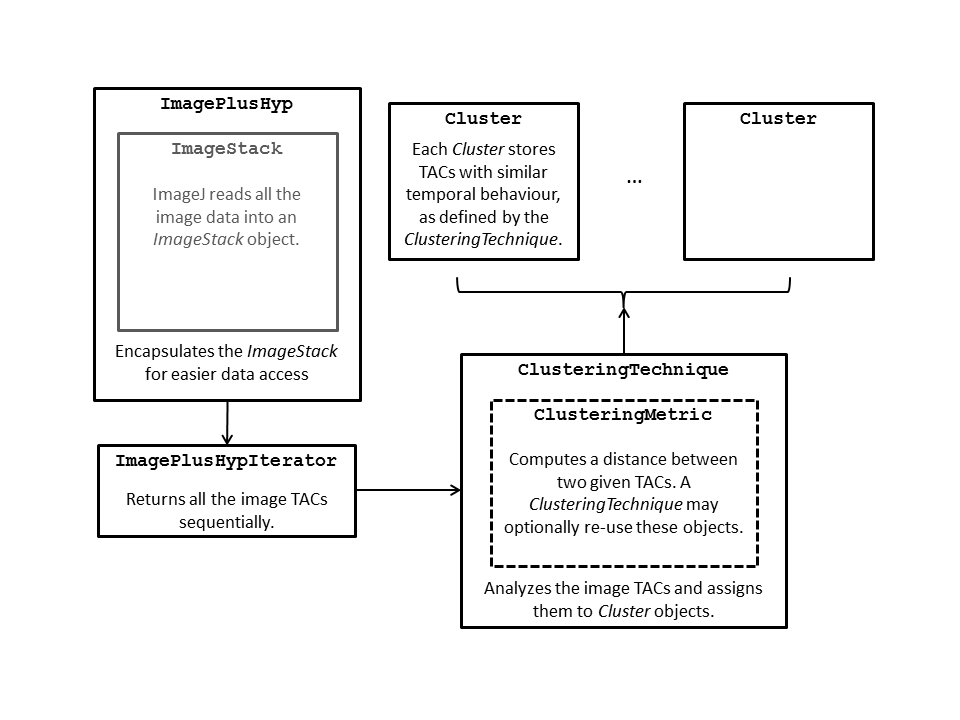
\includegraphics[width=\textwidth]{figures/class_structure}
  \caption{jClustering class structure and relationships.}
  \label{fig:class_structure}
\end{figure}

We can sum up briefly what the presented class structures wants to achieve. As this tool is intended to be used in dynamic images (2D + time or 3D + time), the {\tt ImagePlus} object will contain a {\tt ImageStack} will all the slices and temporal information (ImageJ uses a 3D matrix to store 4D images). As there are no immediate methods to retrieve the time-activity curve (TAC) for a given voxel (that is, the array of different gray scale intensities of that voxel through the time axis), the {\tt ImagePlusHyp} object encapsulates the original {\tt ImagePlus} and adds a {\tt getTAC(int x, int y, int slice)} method that allows to access that data very easily. However, the direct use of {\tt getTac} {\bf is strongly discouraged}. Instead, this object implements the {\tt Iterable} interface using the {\tt ImagePlusHypIterator} class and returns, one by one, all the voxels in the image using objects of the class {\tt Voxel}, which includes the original voxel coordinates and the TAC as publicly accessible class fields. 

This iterator will check whether a given voxel has been masked (the value is 0.0 through all the frames) and will not return it, diminishing the complexity of the clustering problem to solve\footnote{Utilities for masking dynamic studies have been published as part of the LIM tools ImageJ plugin available at \url{https://github.com/HGGM-LIM/limtools}. The particulars of this process are outside the scope of this document.}. In any case, you are free to use the {\tt getTAC(int x, int y, int slice)} method at your own risk.

If you want to implement a new clustering technique using jClustering, it is very likely you only need to extend the {\tt ClusteringTechnique} abstract class. This class provides the necessary methods for the clustering operation as well as references to the objects that will be used to represent the different clusters (via an array of {\tt Cluster} objects). If you want instead
to implement a function that computes the distance between two given TACs and that can be reused between different {\tt ClusteringTechnique} objects, extend the {\tt ClusteringMetric} class instead.

\section{Implementing a {\tt ClusteringTechnique}}
\label{sec:clustmet}

The {\tt ClusteringTechnique} abstract class contains internal references to the following objects:

\begin{itemize}
\item An {\tt ImagePlusHyp} named {\tt ip}. This is the main object you are going to read data from (typically via the provided {\tt ImagePlusHypIterator}).

\item A {\tt ClusteringMetric} named {\tt metric}. Depending on the type of algorithm that you are implementing, you might not need to worry about this reference. Currently, the only implementation that uses different distances is k-means.

\item A {\tt JPanel} named {\tt jp}. If you need to implement some configuration options, this is the object that you need to use to add different GUI elements.

\item An {\tt ArrayList<Cluster>} named {\tt clusters}. This object has already been initialized for you and you only need to add new {\tt Cluster} objects to it. 
\end{itemize}

There is only one method that you {\bf must} implement in your algorithm: {\tt process()}. This method must fill in the {\tt clusters} object according to your local algorithm. Also, your class must belong to the {\tt jclustering.techniques} package in order to be found by the automatic class detection algorithm (see section \ref{sec:automatic_class} for more information on this).

Check the code example shown on listing \ref{clustech1}. It provides a very simple algorithm consisting on grouping together those voxels with TACs that peak at the same time.

\lstinputlisting[caption={Your first {\tt ClusteringTechnique}.}, label=clustech1]{code/sample_technique1.java}

This code uses the {\tt getMaxIndex(double [] tac)} method from the {\tt jclustering.MathUtils} class, which provides misc mathematical utilities. This method returns the index of the {\tt tac} array that contains the maximum value. With this value (plus $1$, as there is no cluster 0), we can call the method {\tt addTACtoCluster(Voxel v, int n)}, that automatically takes care of the rest of the cluster addition process.

In case we want to add a selector in order to use some of the existing metrics (which we can then access through the {\tt metric} object), we only need a little extra bit of code (check Listing \ref{clustech2}) as there is an {\tt addMetricsToJPanel(JPanel jp)} method that takes care of most of the operation. Other GUI components must be fully implemented to work (though there are several static helper methods in the {\tt GUIUtils} class.

\lstinputlisting[caption={A {\tt ClusteringTechnique} that includes a {\tt ClusteringMetric} selector.}, label=clustech2]{code/sample_technique2.java}

\subsection{Returning additional information}
\label{subsec:clustech_additional}

After the {\tt clusters} object has been correctly filled, jClustering takes care of everything else and saves the results to a file and shows the resulting clusters on screen (please refer to the user manual for more information on this). However, this approach might not be enough for all the information that we want to provide after our algorithm finishes.

Consider the PCA {\tt ClusteringTechnique} implementation (\url{https://github.com/HGGM-LIM/jclustering/blob/master/src/main/java/jclustering/techniques/PCA.java}). This technique shows an additional image on screen; it uses the very specific {\tt RealMatrix2IJ(RealMatrix rm, int [] dim, ImagePlusHyp ip, boolean skip\_noisy, String name)} method, but any {\tt ImagePlus} object can be created and shown on screen at any point during the {\tt process()} implementation. 

However, it also stores in a file additional information (in this case, the values of the principal components found). Internally, the {\tt ClusteringTechnique} class also contains the object {\tt String [] additionalInfo}, which defaults to a {\tt null} reference. If this algorithm needs to save on file some extra numerical values, this is the string that needs to be used. Consider the following code sample from the {\tt PCA.java} file (code listing ):

\lstinputlisting[caption={Code sample that allows to save extra information}, label=clustech3]{code/sample_technique3.java}

This string array is expected to be of even length. The $i$ positions contain the initial name of the file (it will be completed using a timestamp and the {\tt .txt} extension) and the $i+1$ contain the actual information that will be saved to that file.

\section{Implementing a {\tt ClusteringMetric}}
\label{sec:clustmet}

A {\tt ClusteringMetric} is used inside a {\tt ClusteringTechnique} that calls internally the methods of its {\tt metric} object. It is a very simple object used to compute the distance between two given TACs while at the same time allow for future code reusing. Currently, only the k-means implementation allows to use different metrics.

The only method that {\bf must} be implemented is {\tt double distance(double [] a, double [] b)}, which returns the distance between TACs {\tt a} and {\tt b}. There is a {\tt void init()} method that can be used as a constructor to initialize the objects that will be used in each {\tt distance} call.

As a sample, let's take a look at the correlation implementation (\url{https://github.com/HGGM-LIM/jclustering/blob/master/src/main/java/jclustering/metrics/Correlation.java}) in code listings \ref{clustmet1}.

\lstinputlisting[caption={{\tt Correlation} metric.}, label=clustmet1]{code/sample_metric1.java}

As you can see, this implementation uses the {\tt init()} method to initialize the {\tt PearsonsCorrelation} object that is used in the calls to {\tt distance}. This method is called just once when the {\tt ClusteringMetric} is initialized inside the {\tt ClusteringTechnique}.

\section{Automatic class detection}
\label{sec:automatic_class}

Techniques and metrics are added automatically to their respective selectors thanks to class autodetection methods ({\tt getClusteringTechnique} and {\tt getClusteringMetric} in {\tt Utils.java} (\url{https://github.com/HGGM-LIM/jclustering/blob/master/src/main/java/jclustering/Utils.java})). This allows new developers to implement directly their own classes and they will be available from the main window the next time jClustering is run.

\section{Behavior of the {\tt Cluster} object}
\label{sec:cluster_behavior}

The {\tt Cluster} object behaves in two different ways depending on how it is initialized. This reflects the two different ways it may work during an iterative clustering process:

\begin{enumerate}
\item The centroid for the cluster may be fixed at creation time and does not change when a new voxel is added.
\item The centroid for the cluster is modified with each voxel addition.
\end{enumerate}

The first behavior is characteristic of k-means, for instance, while the second one belongs to other approaches such as leader-follower. In order to avoid implementing two different {\tt Cluster} objects, it was decided that the constructor would define how this object behaves.

\begin{enumerate}
\item If the constructor is called with a {\tt double []} parameter that represents the centroid TAC, it will be fixed.
\item If the constructor is called with no parameters or with a {\tt Voxel} object, the centroid will be modified with each addition, computing the new mean TAC.
\end{enumerate}

\section{Reference}
\label{sec:reference}

Mateos-Pérez JM, García-Villalba C, Pascau J, Desco M, Vaquero JJ (2013) jClustering, an Open Framework for the Development of 4D Clustering Algorithms. PLoS ONE 8(8): e70797. doi:10.1371/journal.pone.0070797. Available at
\url{http://www.plosone.org/article/info\%3Adoi\%2F10.1371\%2Fjournal.pone.0070797}.



\end{document}